\chapter{Arquitectura del sistema}
\label{cap:arquitectura}

En este capítulo se describe la arquitectura del sistema desarrollado. El sistema completo tiene tres grandes  objetivos principales: la detección en tiempo real de sismos en Chile y en el mundo, la presentación de la información a los usuarios en tiempo real y el almacenamiento de datos históricos que permitan realizar otros estudios relacionados.

\begin{figure}[h]
	\centering
	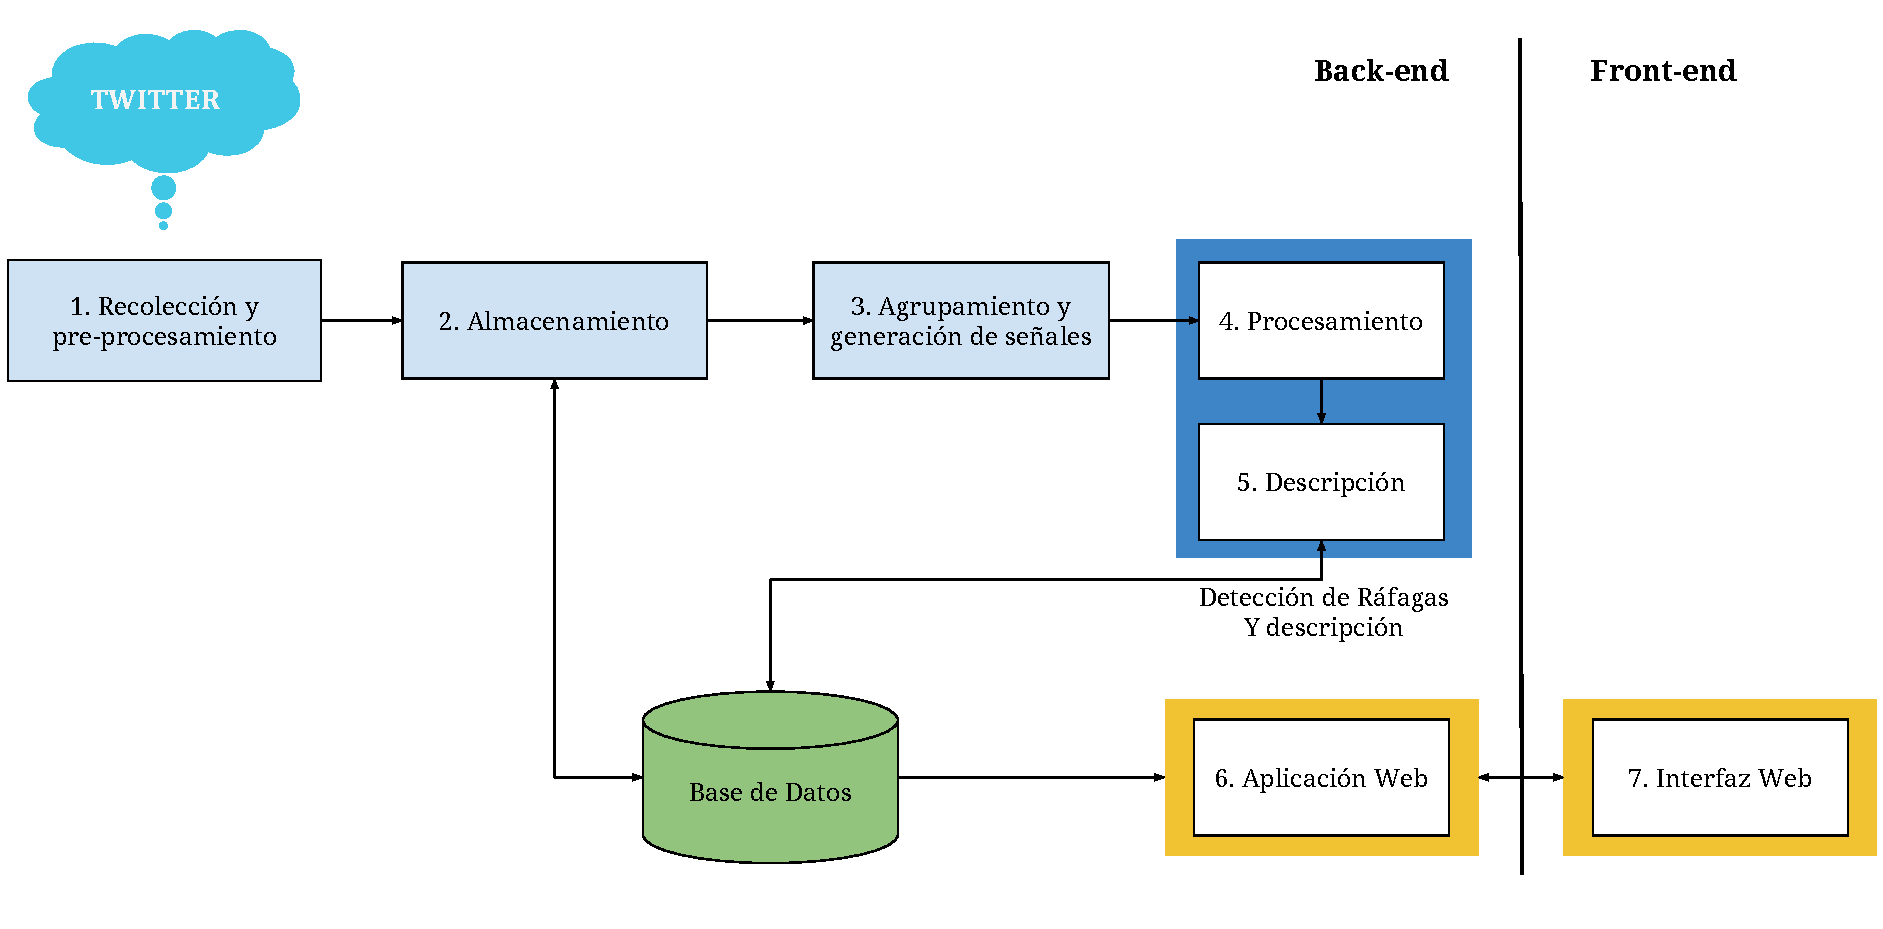
\includegraphics[width=\linewidth]{imagenes/Arquitectura.pdf}
	\caption{Arquitectura del sistema completo}
	\label{img:arquitectura}
\end{figure}

La figura \ref{img:arquitectura} es un esquema de los módulos que conforman el sistema y la forma en que cada uno interactúa con los demás. 
%
Cabe destacar que la experimentación fue una parte importante de este trabajo de tesis, es por esto que algunos de los procesos generan información que fue evaluada durante la etapa de análisis y que, en base a los resultados obtenidos, se tomó la decisión de no incluirla en las visualizaciones de la aplicación Web. 
%
Sin embargo, toda la información generada quedó almacenada en una base de datos en los servidores del Centro de Investigación de la Web Semántica para ser utilizada en investigaciones futuras. 

En las siguientes secciones se explica brevemente la función de cada módulo que compone el sistema.

\section{Recolección de datos y pre-procesamiento}
\label{sec:recoleccion}
El \textbf{módulo 1} se encarga de obtener el flujo de \textit{tweets} a medida que estos son publicados en la red social. Para esto se utiliza la API que provee Twitter para acceder a sus datos y algunos criterios de filtrado. 

\subsection{API de Twitter}

Twitter tiene dos servicios para acceder a los datos públicos: 
%
La API de búsqueda, que permite realizar consultas usando palabras clave, idioma, coordenadas geográficas, etc. 
%
Y la API para acceder al \textit{stream} público\footnote{\url{https://dev.twitter.com/streaming/public}} y que permite obtener el flujo de \textit{tweets} publicados en tiempo real filtrado por palabras clave, idioma, etc.
%
La principal diferencia entre ambas opciones son las limitaciones, ya que la API de búsqueda permite hacer una cantidad limitada de consultas por minuto y la API para acceder al \textit{stream} limita la muestra de datos entregada para que no exceda al 1\% del total de mensajes publicados en Twitter en ese momento.
% 
Para este caso, a diferencia de Sakaki et al.\cite{sakaki2013tweet}, Robinson et al. \cite{robinson2013sensitive} y Earle et al. \cite{earle2012twitter}, se decidió ocupar la API para acceder al \textit{stream} público, como también lo hacen Avennuti et. al \cite{avvenuti2014earthquake}.
%
Mediante el uso de la API para acceder al \textit{stream} es posible obtener los \textit{tweets} más rápido y detectar en tiempo más cercano al ``tiempo real''. Además, los filtros que se utilizan al obtener los datos disminuyen el número de \textit{tweets} de interés y según nuestra apreciación, la limitante que impone Twitter sobre la muestra de los datos no alcanza a ser suficientemente ajustada como para evitar que se obtengan todos los \textit{tweets} de interés. 

\begin{figure}[h]
	\centering
	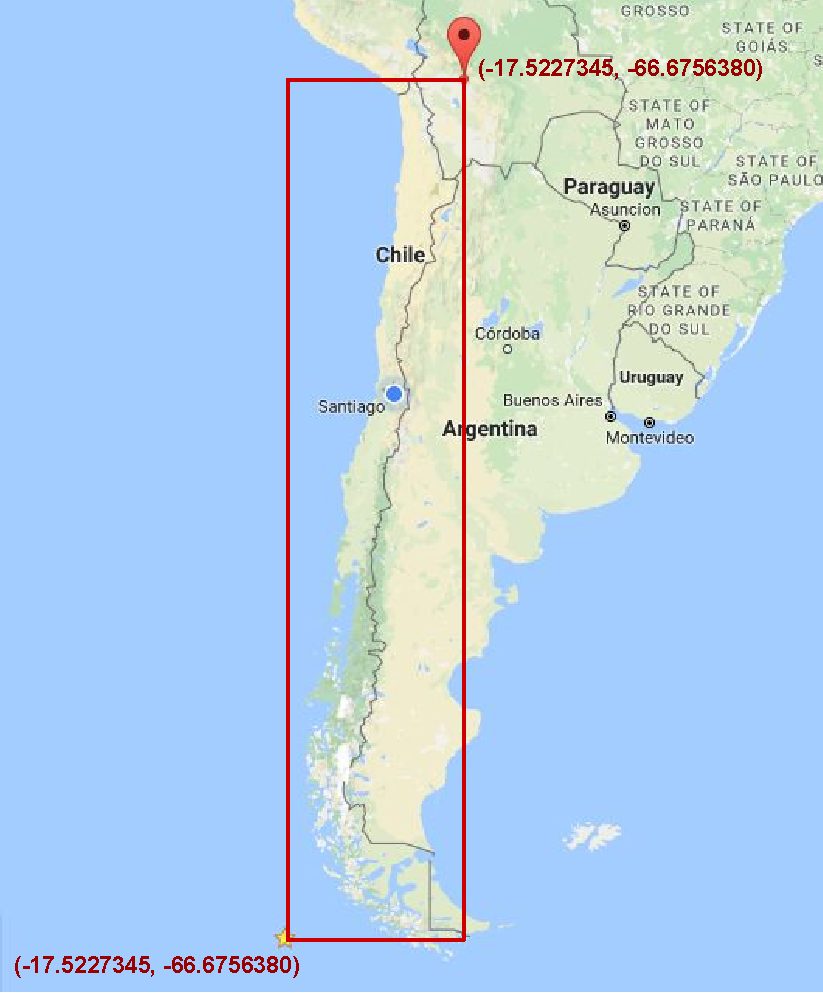
\includegraphics[width=0.5\linewidth]{imagenes/boundingbox.pdf}
	\caption{Cuadro de delimitación geográfica utilizado para complementar la recolección y obtener una mayor cantidad de información geolocalizada de Chile.}
	\label{img:boundingbox}
\end{figure}

\subsection{Criterios de selección de tweets}

Para obtener los datos, se filtró el flujo de mensajes para obtener todos los \textit{tweets} que mencionan alguna de las palabras clave relacionadas con eventos sísmicos. 
%
Las palabras clave corresponden a las traducciones de ``temblor'', ``sismo'' y ``terremoto'' en diferentes idiomas. 
%
La lista completa de palabras clave utilizadas se encuentran listadas en la figura \ref{img:keywords} en el capítulo \ref{cap:analisis}. 
%
Este criterio permite obtener \textit{tweets} provenientes de cualquier parte del mundo.

%
Además del filtro por palabras clave, se agrega un filtro (OR lógico) en forma de cuadro de límite geográfico que rodea todo el territorio nacional, tal como se muestra en la figura \ref{img:boundingbox}.
%
Con este criterio se obtiene una mayor cantidad de mensajes publicados por usuarios chilenos con información de geolocalización que permiten mejorar la caracterización de sismos en Chile.
%
Este filtro se puede modificar o extender para incluir otras áreas geográficas que requieran mayor atención, por ejemplo, otros países con alta sísmicidad. 


Con esta forma de selección se obtiene una muestra representativa de reportes de sismos en el mundo e información más detallada de publicaciones hechas por usuarios en Chile, permitiendo brindar mejor soporte a la detección nacional.


Los \textit{tweets} que conforman el flujo de Twitter no son descartados como en soluciones similares~\cite{avvenuti2014ears}. 
%
Esto significa que \textit{re-tweets} y \textit{tweets} que citan otros \textit{tweets} y que están relacionados con sismos o que se encuentran dentro del cuadro geográfico, son analizados junto con los originales. 
%
Esto hace que las señales a analizar sean más ruidosas, pero aumenta el volumen del flujo de \textit{tweets}, lo que es útil para caracterizar mejor los eventos. 

\subsection{Mensajes en diferentes idiomas}
El alcance mundial que se intenta cubrir trae consigo la dificultad de tener que procesar mensajes que están escritos en diferentes idiomas. 
%
Una tarea crucial para la detección y la descripción de cada evento es la de segmentar las oraciones en palabras.
%
Esta tarea es relativamente simple para casi todos los idiomas cuando se usan los elementos específicos de separación para cada uno (por ejemplo: espacios, puntos, comas, apóstrofes, etc.).
% 
Sin embargo, para idiomas que no utilizan signos de separación es más complejo.
%
Este es el caso del idioma chino, para el cual se utilizó la biblioteca {\em Stanford NLP Chinese Word Segmentation}\footnote{\url{http://nlp.stanford.edu/projects/chinese-nlp.shtml}}.

\subsection{Robots Web y usuarios maliciosos}
\label{subsec:bots}
Algunos usuarios o procesos automáticos son utilizados para reportar periódicamente todos los últimos sismos ocurridos, por ejemplo, a lo largo del día previo. 
%
Al ser de carácter automático, estas publicaciones se hacen seguidas una de otra y en un corto periodo de tiempo. 
%
Este comportamiento puede, erróneamente, ser considerado como una ráfaga de reportes de sismos y ser reportado como una detección falsa.  
%
Usuarios con malas intenciones también pueden utilizar este mecanismo para difundir un rumor. 
%
Para evitar este problema, al momento de recolectar los \textit{tweets}, se añade una \textit{etiqueta} a los \textit{tweets} publicados por el mismo usuario en un periodo inferior a 5 minutos desde que publicó el mensaje previo, para luego no considerarlos en la detección. 
%
Si ocurre un sismo, se espera que este sea reportado por varios usuarios en la misma ubicación geográfica, por lo que la detección no se verá afectada por este filtro.

%
%Para obtener los datos se utiliza la API para acceder al \textit{stream} público de Twitter\footnote{\url{https://dev.twitter.com/streaming/public}} y una librería en Java\footnote{\url{http://twitter4j.org/}} que integra el servicio con la aplicación.
%
%Los datos se reciben en formato JSON\footnote{\url{https://dev.twitter.com/docs/tweet-entities}}.

\subsection{Procesamiento de los mensajes}
Los \textit{tweets} recolectados reciben un primer procesamiento encargado de agregar metadatos a partir del texto y de otras características del \textit{tweet}. El pre-procesamiento de los datos incluye:
\begin{itemize}
\item La ejecución del algoritmo SentiStreigth\footnote{\url{http://sentistrength.wlv.ac.uk}} para calcular el sentimiento del mensaje.
\item La búsqueda de menciones de nombres de países en diferentes idiomas en el mensaje y en los campos que incluyen información de localidad del usuario. En el resto del documento nos referimos a este proceso como proceso de geolocalización.
\item Etiquetado de \textit{tweets} de carácter posiblemente malicioso o casos particulares que perturban el correcto funcionamiento de la detección, como se describió en anteriormente en \ref{subsec:bots}.%Se marcan los \textit{tweets} publicados por el mismo usuario en un lapso menor a 5 minutos y también \textit{tweets} publicados por usuarios incluidos en una lista negra. La lista negra existe para casos particulares en que se detecten usuarios cuyas publicaciones entorpezcan el correcto funcionamiento de la aplicación (como fue el caso de una cuenta mexicana que todos los días publicaba la lista completa de sismos del día anterior). Esta lista puede ser actualizada sin necesidad de interrumpir los procesos. 
\end{itemize}

Los metadatos añadidos fueron parte importante del análisis experimental desarrollado. Se detalla un poco más sobre el proceso de extracción de sentimiento y sobre el proceso de geolocalización en el capítulo \ref{cap:procesamiento}. Además en el capítulo \ref{cap:analisis} se explica cómo se utilizaron estos datos en el análisis experimental y los resultados obtenidos.

Finalmente, luego de procesar cada \textit{tweet}, este es puesto en una cola en memoria RAM para ser utilizado por el módulo 2.

\section{Almacenamiento de datos}

\begin{figure}[ht]
	\centering
	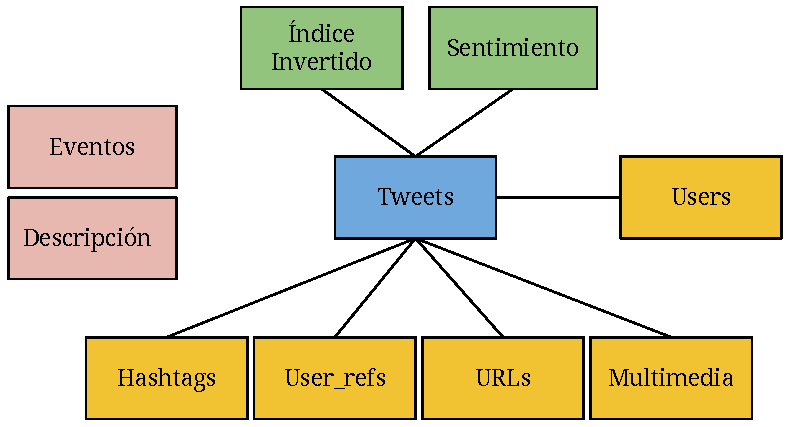
\includegraphics[width=0.8\linewidth]{imagenes/tweetmodel.pdf}
	\caption{Modelo de las tablas generadas diariamente que conforman la base de datos.}
	\label{img:database}
\end{figure}

El \textbf{módulo 2} se encarga del almacenamiento de los \textit{tweets} recolectados y los metadatos asociados. La información se almacena en una base de datos relacional MySQL. 
%
Cada día se crean nuevas tablas para almacenar la información. Esta medida busca evitar tablas de gran tamaño y así optimizar los tiempos de búsqueda en la base de datos. 


La imagen \ref{img:database} muestra las tablas generadas diariamente. 
%
Las tablas de color amarillo almacenan información relacionada al \textit{tweet}. 
%
Los campos de estas tablas guardan información, en su mayoría, proveniente directamente desde Twitter.
%
Algunos de los datos almacenados en estas tablas son generados en el módulo de pre-procesamiento, como la información de geolocalización y una etiqueta que indican si el \textit{tweet} fue publicado por un mismo usuario en un corto periodo de tiempo.

Las tablas de color verde almacenan otra información generada por el sistema.
%
Una de ellas almacena un índice invertido de las palabras que conforman el texto de los \textit{tweet} y la otra almacena el resultado del análisis de sentimiento para cada \textit{tweet}. 
%
Las tablas de color rosado almacenan la información relacionada con las detecciones y son pobladas con la información generada en los módulos 4 y 5 que se describen más adelante. 


Además de las tablas del modelo de la figura~\ref{img:database}, existen otras ``tablas virtuales'' o ``vistas'' destinadas al almacenamiento de datos agregados que son utilizados para la detección de ráfagas y para el almacenamiento de datos precalculados para las visualizaciones.
%
%En el \nameref{anexo:bd} se detalla el esquema de la base de datos y los campos que conforman cada tipo de tabla creada.

\section{Agrupación de \textit{tweets} y generación de señales}

El \textbf{módulo 3} se encarga de preparar los datos para ser procesados en busca de ráfagas.
%
Los \textit{tweets} del \textit{stream} son agrupados en conjuntos etiquetados según el \textit{timestamp} de la fecha de creación. 
%
Cada conjunto de \textit{tweets} representa una ventana de tiempo individual. 
%
Las ventanas de tiempo son alineadas secuencialmente.
%
Cada secuencia de ventanas puede ser representada como una señal discreta, la que es analizada por el módulo siguiente.
%
Como parte de la experimentación se generaron diferentes tipos de señales a partir de algunos atributos de interés específicos. %Por ejemplo, señales conformadas por tweets que mencionaban un mismo país en el mensaje. 
%
Las señales generadas fueron:

\begin{enumerate}
\item Señal de \textit{tweets} con palabras clave: Señal conformada por todos los \textit{tweets} que contienen cualquier palabra relacionada con sismos en cualquier idioma~\footnote{Palabras especificadas en una lista de palabras clave.}. 
\item Señales de localización del usuario: Señales construidas mediante la agrupación de \textit{tweets} publicados por usuarios que indican pertenecer al mismo país en su perfil. Esta agrupación se hace considerando los \textit{tweets} que contienen palabras relacionadas con sismos.
\item Señales de localización considerando el texto: Señales construidas mediante la agrupación de \textit{tweets} que mencionan el mismo país en el texto del mensaje. Esta agrupación se hace considerando los \textit{tweets} que contienen palabras relacionadas con sismos.
\item Señales de idioma: Señales construidas mediante la agrupación de \textit{tweets} escritos en el mismo idioma. Para esto se consideran los \textit{tweets} que contienen palabras relacionadas con sismos.
\item Señales de sentimiento: Dos señales, una que agrupa los \textit{tweets} que reportan sismos y que expresan sentimiento positivo y otra con los \textit{tweets} que reportan sismos y que expresan sentimiento negativo. 
\end{enumerate}

En el capítulo \ref{cap:analisis} se vuelve a mencionar las señales creadas y se presentan los resultados obtenidos a partir de su análisis para detección de sismos.

\section{Procesamiento de señales}

El \textbf{módulo 4} se encarga de procesar las secuencias de ventanas generadas por el módulo anterior y analizarlas en busca de ráfagas.  
%
Para analizar los datos se utiliza una estructura de datos de tabla de hash concurrente en donde se almacenan datos estadísticos asociados a cada ventana de tiempo. Esta estructura permite acceder a los datos en paralelo y mejorar el rendimiento.
%
El detalle de la metodología de detección se explicó previamente en el capítulo \ref{cap:deteccion}.

\section{Descripción de los eventos detectados}

El \textbf{módulo 5} se encarga de la descripción de eventos, es decir, se encarga de procesar la ventana de tiempo donde se detectó una ráfaga para determinar las palabras y los \textit{tweets} que propiciaron ese comportamiento.
%
Con esta información se complementa la información temporal y geográfica asociada a esa ventana de tiempo.
%
En conjunto toda esta información describe un evento, ya que responden a las preguntas sobre el cuándo, dónde y qué es lo que pasó específicamente en cada evento detectado.
%
En el capítulo \ref{cap:casos} se muestra un breve análisis para algunos casos de eventos sísmicos detectados  donde se responden a estas preguntas.  


\section{Aplicación Web}

La aplicación Web se compone por dos partes: el servidor Web (módulo 6) y el frontend que se ejecuta en el browser de los usuarios (módulo 7). 

\subsection{Servidor Web}
El \textbf{módulo 6} corresponde al servidor de la aplicación Web implementado en Python utilizando el \textit{framework} Flask\footnote{\url{http://flask.pocoo.org/}}. El servidor accede directamente a la base de datos y consulta los datos a medida que estos van siendo agregados. Para servir los datos en tiempo real se utiliza un caché con auto-refresco de 1 segundo, que evita sobrecargar el servidor cuando acceden muchas personas al mismo tiempo a la aplicación. 

\subsection{Interfaz Web}
El \textbf{módulo 7} corresponde a la interfaz de la aplicación Web. Para su implementación se utilizaron las siguientes bibliotecas:
\begin{itemize}
\item JQuery.js\footnote{\url{https://jquery.com/}}: Biblioteca javascript para facilitar la manipulación de documentos y las llamadas Ajax. 
\item Bootstrap\footnote{\url{http://getbootstrap.com/}}: Framework para desarrollar aplicaciones responsivas y que funcionan en varios dispositivos.
\item D3.js\footnote{\url{https://d3js.org/}}: Biblioteca javascript para manipular documentos basados en datos y generar visualizaciones interactivas. %
\item Leaflet.js\footnote{\url{http://leafletjs.com/}}: Biblioteca javascript para visualizaciones interactivas usando mapas. 
\item Leaflet.heat\footnote{\url{https://github.com/Leaflet/Leaflet.heat}}: Un plugin que extiende Leaflet para crear mapas de calor. 
\item Leaflet.markercluster\footnote{\url{https://github.com/Leaflet/Leaflet.markercluster}}: Un plugin que extiende Leaflet para agrupar marcadores cercanos entre si y desplegarlos de forma interactiva. 
\end{itemize}

%En la sección \ref{sec:visualizacion} se detallan las visualizaciones utilizadas para presentar los datos y en la sección \ref{sec:aplicacion} se muestran vistas completas de la aplicación y su modo de uso. 
En el capítulo \ref{cap:aplicacion} se detallan las visualizaciones utilizadas para presentar los datos, así como también, vistas completas de la aplicación y su modo de uso. 